%*********************************************************
\section{Introduction to the non-linear optics} 
%*********************************************************


%*********************************************************
\subsection{What is non-linear optics?}
When you immerse a solid, either an insulator or a semiconductor, in an electric field (see Fig. \ref{immerse}), the dipoles inside the material get orientated along the field lines and create an internal field, 
\begin{wrapfigure}{r}{0.5\textwidth}
  \begin{center}
    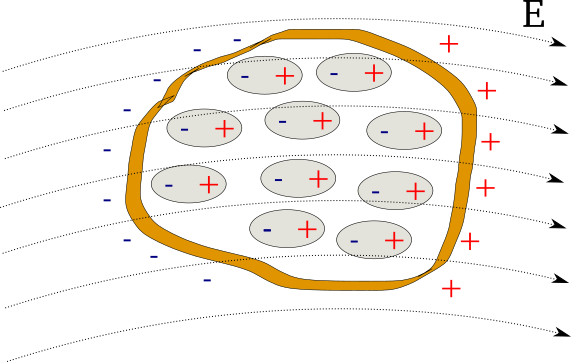
\includegraphics[width=0.4\textwidth]{Figures/immerse}
  \end{center}
  \caption{A solid immersed in an electric field. \label{immerse}}
\end{wrapfigure}
the \emph{polarisation} $\PPc$, opposite to the field that generates it. This naive picture, even if valid only for finite systems, gives us an idea of the effect of an external electric field on a material.
The \emph{total electric field} inside the solid $\EEc(\rr,t)$ is the sum of the external plus the polarisation one:
\be
\EEc(\rr,t) = \DDc(\rr,t) - \PPc(\rr,t),
\label{materialeq}
\ee
where $\DDc(\rr,t)$ is the \emph{electric displacement}.
This equation is one of the so-called  ``materials equations", namely the Maxwell equations for electric and magnetic fields in bulk materials. %and $ \EEc(\rr,t)$ is the Total Electric Field. %In order to understand the origin of these two fields, it is possible to write down their corresponding Gauss's equations: 
%\ben
%\nabla \DDc(\rr,t)  = \frac{\rho_{ext}(\rr,t)}{\epsilon_0} \mbox{ , } \nabla \EEc(\rr,t)  = \frac{\rho_{tot}(\rr,t)}{\epsilon_0}. 
%\een
%From the above equations one can see that the Electric Displacement is generated by the external charges while the Electric Field is due to the sum of external plus the internal ones, namely the total charge. This explains the structure of Eq.~\ref{materialeq} being the total field equal to the external one minus the polarisation that is the field generated by the internal charges and  opposed to the external one. 
In general one can expand the polarisation  $\PPc$ in a power series of the total electric field $\EEc$: 
\be
\PPc = \PPc_0 + \chi^{(1)} \EEc + \chi^{(2)} \EEc^2 + \chi^{(3)} \EEc^3 + ....
\label{pexpansion}
\ee
where $\PPc_0$ is the intrinsic polarisation of the material at zero electric field, and the coefficients $\chi^{(1)}, \chi^{(2)},...$ are response functions of increasing order. Equation~\ref{pexpansion} is valid for a wide range of situations. However, there are cases where this expansion fails: 1) for very strong fields, beyond the convergence radius of the expansion\cite{lee2014first}; 2) when there is an hysteresis, and therefore there is not a univocal relation between polarisation and electric field; 3) close a to phase transitions, where a small external field can drastically change the material properties. In this highlight, we will restrict to the cases in which the expansion in Eq.~\ref{pexpansion} is valid.\\ 
%Moreover in the present work we will always assume $\PPc_0=0$ because we are not interested in materials with intrinsic polarisation as for instance ferroeletrics.\\
%\begin{figure}[ht]
%  \begin{center}
%    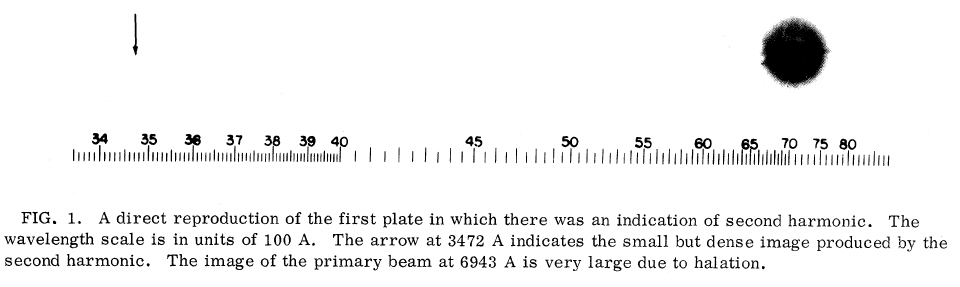
\includegraphics[width=0.9\textwidth]{Figures/SHG_franken.png}
%  \end{center}        
%  \caption{The original photographic image of the SHG with the corresponding caption from the Franken's paper\cite{franken1961generation}. \label{frankenfig}} % (Onestly I don't see anything below the arrow)
%\end{figure}
%Now we introduce the concept of non-linear optics. 
The first term $\chi^{(1)}$ of the power series describes all the phenomena which belong to the linear optics regime. All the other terms  $\chi^{(2)}, \chi^{(3)},.... $  describe the non-linear response, that will be the topic of this highlight. \\
What does non-linear response mean in practice? We can gain an understanding by rewriting Eq.~\ref{pexpansion} in frequency domain. For an homogeneous material we obtain:
\be
\PPc(\omega) = \chi^{(1)} (\omega) \EEc(\omega)  + \chi^{(2)} (\omega = \omega_1 + \omega_2) \EEc(\omega_1) \EEc(\omega_2) + ....
\label{pexpomega}
\ee
In the first term (linear regime) on the RHS, the outgoing light [i.e. the polarisation $\PPc (\omega)$] has the same frequency $\omega$ of the incoming one [i.e. the electric filed $\EEc (\omega)$]. On the contrary, terms beyond the first one contain frequency sum or frequency difference terms, for which the outgoing light has a different frequency (or colour) from the incoming one.  For example, in the second harmonic generation (SHG), the outgoing light has a frequency that is twice that of the incoming one. \\
This effect, despite evident from the equation, is not something we observe in our everyday lives. In fact, the non-linear coefficients of the polarisation expansion are extremely small. In order to obtain a detectable non-linear response, one needs a sufficiently strong light source. For this reason, the first experimental measurement of second-harmonic generation (SHG) dates 1961~\cite{franken1961generation}, a year after the laser invention.~\cite{maiman1960stimulated} In this first experiment of non-linear optics, Franken and his collaborators were able to obtain a SHG signal from a ruby crystal employing a monochromatic laser beam with an intensity of $10^5$ volts/cm.\\ % see Fig.~\ref{frankenfig}.\\
Nowadays lasers with an intensity equivalent to the one used in the Franken's experiment are commercially available in shops and SHG is a common technique to double the laser frequency.\\
Of course, non-linear optics is not limited to the SHG. Nonlinear order terms cover a large spectra of phenomena, such as optical saturation, sum frequency generation, two-photon absorption, generation of higher harmonics. In the next section we will show some applications of non-linear response, and then how these applications can be described from first-principles.
%taken away: high harmonic and so on => this is a phenomenon where the expansions do fail!!!!!

%*********************************************************
\subsection{What can be done with non-linear optics?} 
\begin{wrapfigure}{r}{0.5\textwidth}
  \begin{center}
    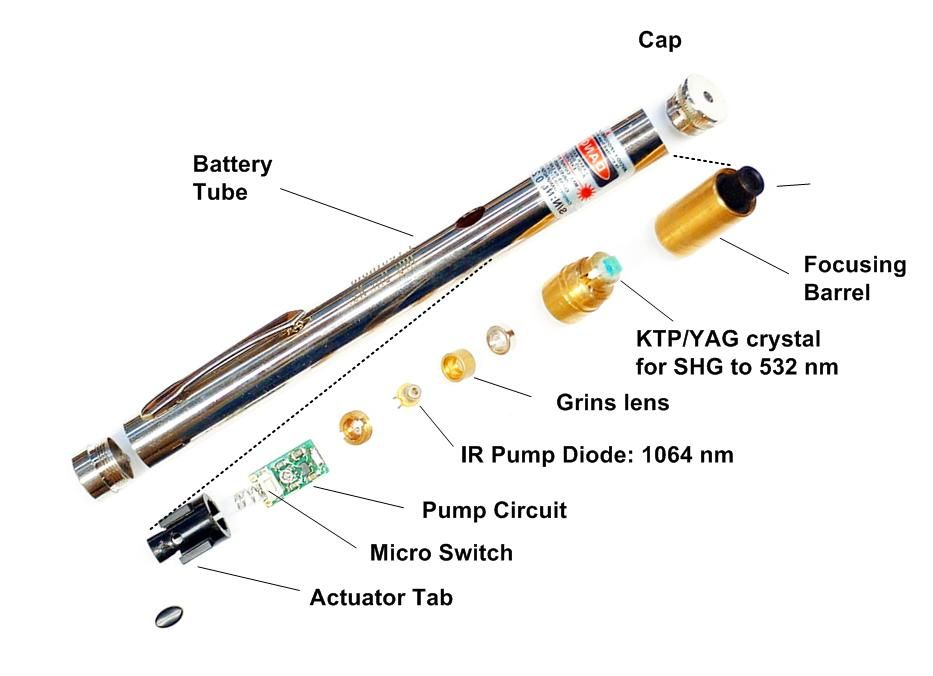
\includegraphics[width=0.4\textwidth]{Figures/lasergreen}
  \end{center}
  \caption{Schematic of the green laser pointer. \label{greenlaser}}
\end{wrapfigure}
In the last thirty years, the field of non-linear spectroscopy~\cite{bloembergen1982nonlinear} made progresses in leaps and bounds. One of the most common commercial application is the green laser pointer. Many of us uses it when giving slideshow presentations. In this device, the green light is obtained combining a (infra)red laser with a non-linear crystal that doubles the frequency (see Fig.~\ref{greenlaser}). Nowadays non-linear crystals are routinely used in laboratories to change shape, length and intensity of laser beams. \\
%              \begin{wrapfigure}{l}{0.4\textwidth}
%    \vspace{-0.7cm}
%  \begin{center}
%    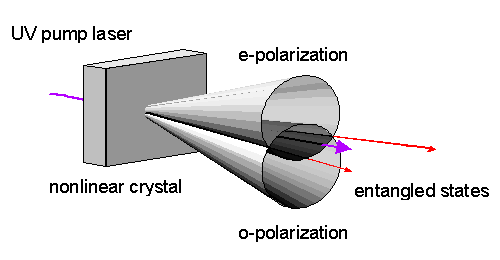
\includegraphics[width=0.4\textwidth]{Figures/entangled}
%  \end{center}
%  \caption{Entangled photons generation. \label{entangled}}
%\end{wrapfigure}
Applications of non-linear optics span a range of disciplines that encompasses condensed matter physics, quantum optics, optoelectronics and medicine.\\

In biomedical research, SHG is used to probe protein dynamics in biological tissues. In fact,  biological tissues does not present a SHG, so nanocrystals with a strong SHG can be bounded to proteins and then inserted in living systems. Under intense illumination, such as the focus of a laser-scanning microscope, these SHG nanocrystals modify the light colour and they can be imaged by means of the two-photon microscopy. Scientists can then visualise the dynamics of the proteins thanks to the nanocrystals. Unlike commonly used fluorescent probes, SHG nanoprobes neither bleach nor blink. The resulting contrast and detectability of SHG nanoprobes provided therefore unique advantages for molecular imaging of living cells and tissues. \cite{pantazis2010second}\\
%
%%\begin{wrapfigure}{l}{0.4\textwidth}
%  \begin{center}
%    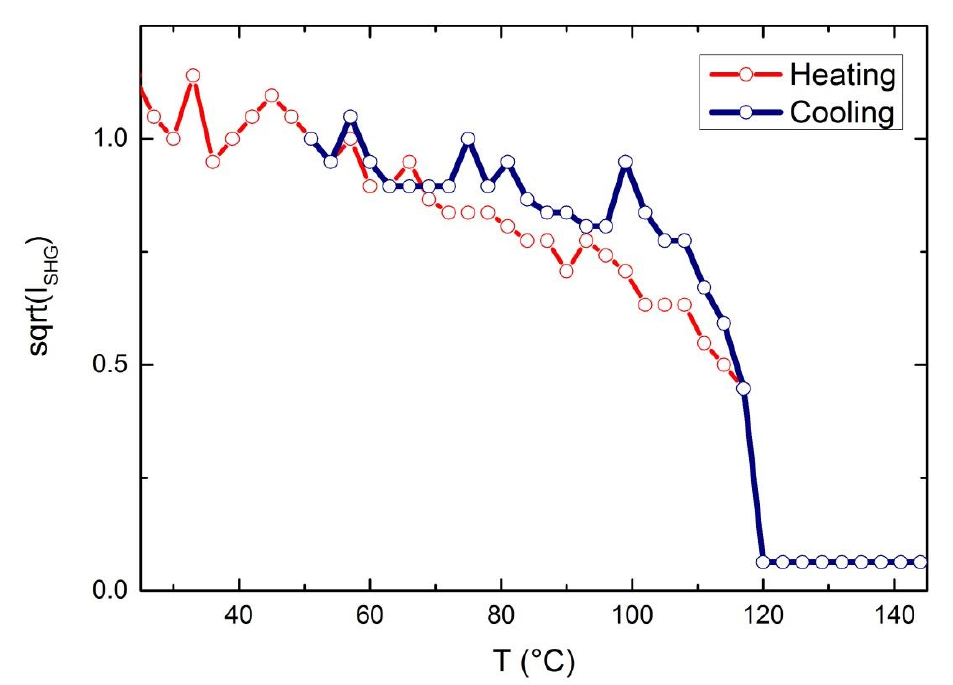
\includegraphics[width=0.4\textwidth]{Figures/ferroelectric}
%  \end{center}
%  \caption{Square root of SHG signal changing due to temperature variation, in a BaTiO$_3$ crystal. \label{ferroelectric}}
%\end{wrapfigure}
%They become a tool .

In quantum optics, non-linear crystals are used to create entangled photons: a high energy photon is transformed in two (or more) lower energy (entangled) photons by means of reverse second- or third-harmonic generation. These photons are used in quantum information studies, quantum cryptography or for quantum computation, due to their entangled states.\cite{PhysRevLett.75.4337}\\ 
%(see Fig.~\ref{entangled}).\cite{PhysRevLett.75.4337}\\

In condensed matter the non-linear response remains an essential tool to characterise and explore electronic and structural properties of materials. 
For example, since second-harmonic generation is present only in materials that lack of inversion symmetry, it became a tool to probe phase transitions and phenomena the break this symmetry. Symmetry inversion can be broken in presence of a macroscopic electric field as the one of piezoelectrics, pyroelectrics, and ferroelectrics, or a bulk magnetization as in ferromagnets. Temperature dependent SHG measurement can be used to discriminate between the different phases of these materials. %In Fig.~\ref{ferroelectric} it is shown how the SHG signal changes with the temperature in the ferroelectric BaTiO$_3$. At 120\degree~C there is no more signal and the change is very abrupt. 
%This confirms that 120\degree~C is the temperature where inversion symmetry is restored in BaTiO$_3$ crystal as it loses its ferroelectric properties.\\
%\begin{wrapfigure}{r}{0.4\textwidth}
%  \begin{center}
%    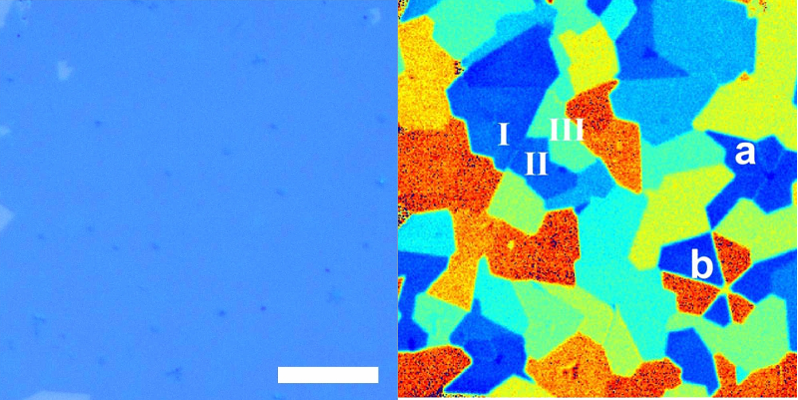
\includegraphics[width=0.4\textwidth]{Figures/mos2}
%  \end{center}
%  \caption{On the left a linear optics image of a  MoS$_2$ single layer. On the right SHG image of the same layer. \label{mos2} [Figure from Ref.\cite{yin2014edge}]}
%\end{wrapfigure}
\begin{wrapfigure}{r}{0.4\textwidth}
 \vspace{-0.8cm}
\begin{center}

\includegraphics[width=0.4\textwidth]{Figures/selffocus}
\end{center}
\vspace{-0.5cm}
\caption{A schematic representation of the self-focusing phenomena in optical fibers. \label{selffocusing}}
\end{wrapfigure}           

Another domain where SHG plays a major role is surface spectroscopy. Experimentally, it is non trivial to disentangle bulk and surface contribution from a given signal. SHG is one of the few techniques that can probe the surface, without contributions from the bulk. The reason lies in the fact that in solids with inversion symmetries the bulk has zero SHG signal. This is true not only for bulk materials but also for liquids that are on average symmetric, with the exception of the liquid-liquid or gas-liquid interfaces. SHG is very sensitive to lattice orientation which can be used to characterise surfaces and interfaces and provides great insights on the surface structures, that sometime are difficult to probe with other techniques.\cite{eisenthal1996liquid}\\

Surface SHG spectroscopy techniques have been applied to characterise two-dimensional (2D) material. In a recent experiment,~\cite{yin2014edge}  X. Yin et al. used this idea to develop a nonlinear optical imaging technique that allows a rapid and all-optical determination of the crystal orientations in 2D materials at a large scale. %In Fig.~\ref{mos2} one sees the main results of  X. Yin et al., on the left there is an image of a single-layer of MoS$_2$ in linear optics and on the right a SHG image of the same layer, where the different colours represent different intensity of the SHG response. The flakes and their orientation are clearly visible in the SHG image.
Further, Y. Li at al. used SHG to probe the number of layers deposited on a surface, using the fact that an even number of layers posses inversion symmetry while an odd one does not.\cite{doi:10.1021/nl401561r} The importance of non-linear response for materials characterization is not limited to the SHG. Also other response functions find applications in condensed matter physics. For example two-photon absorption, that is proportional to the imaginary part of the $\chi^{(3)}$, can be used to probe excited states that are dark in linear optics.\cite{wang2005optical,cassabois2015hexagonal}\\

Finally, nonlinear optics effects can be detrimental for some technologies, limiting their application. For example, self-focusing limits the light power that can be transported by optical fibers. Self-focusing is a non-linear optical process seen in materials exposed to intense electromagnetic radiation due to the third-order response $\chi_3$:  a medium whose refractive index is significantly modified by the third-order response acts as a focusing lens for an electromagnetic wave characterised by an initial transverse intensity gradient, as the one generated by a laser beam (see Fig.~\ref{selffocusing}). The peak intensity of the self-focused region keeps increasing as the wave travels through the medium, until medium damage interrupts this process. At present no solution is known for increasing the self-focusing limit in optical fibers~\cite{encylaser}.\\
In this introduction we covered a minimal part of the positive and negative non-linear phenomena in research and applications, for a general overview different books and reviews are available in literature.\cite{boyd,bloembergen1982nonlinear}

%**********************************************************
\section{How to calculate non-linear response}
\subsection{Response-based and real-time approaches}
The first calculation of non-linear optical response in solids based on quantum mechanics used a density matrix formalism.\cite{bloembergen1964quantum} The latter formalism had been already used to derive local field effects in linear optics\cite{PhysRev.126.413,wiser1963dielectric}, to investigate  saturation of microwave resonances\cite{karplus1948note}, and to describe nuclear magnetic relaxation\cite{kubo1954general,RevModPhys.33.249,PhysRev.102.104}. One advantage of the density matrix formalism is that effects due to the environment, such as dephasing processes, are easy to include.\cite{manzano2020short}

The density matrix formalism is based on the solution of the Liouville-von Neumann equation~\cite{neumann} for the electronic one-body reduced density-matrix $\rho$:
\be
i \hbar \frac{\partial \rho}{\partial t} = [ \HH_A, \rho] + [ \HH_{coh}, \rho] + i\hbar \left ( \frac{\partial \rho}{\partial t} \right )_{damping}.
\label{eomsimple}
\ee
The right-hand side of this equation of motion (EOM), Eq.~\ref{eomsimple}, contains three terms. $\HH_A$ describes the unperturbed energy levels of the system, $\HH_{coh}$ describes the coupling with the external perturbation---which in the case of nonlinear response calculations, is a monochromatic ever lasting electro-magnetic field---and finally $\left ( \partial \rho/\partial t \right )_{damping}$ introduces decoherence and relaxation processes.

%Within a non-interacting approximation for the electron, 
Decoherence is due to the interaction with other degrees of freedom---for example the vibrations of the lattice, or phonon modes---and other environmental effects. The coupling with the environment can be modeled, for example, by introducing a $\HH_{random}$ Hamiltonian which accounts for random processes.\cite{manzano2020short}\\
If one wants to include electron-electron interaction  in the EOM [Eq.~\ref{eomsimple}] static electron correlation can be accounted by a term which has the form $[\Sigma^{xc,static},\rho]$, thus affecting the electronic structure of the system, while dynamical correlation is included as an additional relaxation process in the $\left ( \partial \rho/\partial t \right )_{damping}$ term.
%In the literature different phenomenological models have been proposed for the damping therm, the simplest one is:

%\be

%\left ( \frac{\partial \rho}{\partial t} \right )_{damping} = - \left (\Gamma \rho + \rho \Gamma \right ).

%\label{dmeq}

%\ee

%Where the anti-commutator on the RHS is generated by the non-Hermitian part of the Hamiltonian.\cite{tokman}\\
A steady-state solution for Eq.~\ref{eomsimple} in ascending powers of the coupling term may be found from the following hierarchy equations:
\bea \label{eq:hierDM}
i \hbar \frac{\partial \rho^{(0)}}{\partial t} &=& [ \HH_A, \rho^{(0)}] +  i\hbar \left ( \frac{\partial \rho^{(0)}}{\partial t} \right )_{damping},\\ 
i \hbar \frac{\partial \rho^{(1)}}{\partial t} &=& [ \HH_A, \rho^{(1)}] + [ \HH_{coh}, \rho^{(0)}] + i\hbar \left ( \frac{\partial \rho^{(1)}}{\partial t} \right )_{damping}, \\
i \hbar \frac{\partial \rho^{(2)}}{\partial t} &=& [ \HH_A, \rho^{(2)}] + [ \HH_{coh}, \rho^{(1)}] + i\hbar \left ( \frac{\partial \rho^{(2)}}{\partial t} \right )_{damping}. 
\eea
The first equation gives the density matrix at equilibrium. The second equation describes the linear response. By Fourier analysis it is easy to show that $\rho^{(1)}$ must contain the same frequencies as $\HH_{coh}$. The $\rho^{(2)}$  is the first non-linear term. Differently from $\rho^{(1)}$,  $\rho^{(2)}$ oscillates at a frequency that can be the sum or difference of the incoming fields. This term describes for example, second harmonic generation and optical rectification. %% and the dc term -- commented out as it is not clear to me what are you referring to... is that induced DC current in metallic systems?  
Higher order terms $\rho^{(n)}$, describes for example, higher harmonic generations and saturation phenomena.

From these hierarchy equations, it is possible to derive the corresponding Dyson-like equations for the response functions $\chi^{(1)}$, $\chi^{(2)},\dots$ by differentiating the density matrix respect to the external perturbation. Alternatively, expressions for nonlinear response functions can be also derived directly from perturbation theory.\cite{PhysRevB.56.1787,PhysRevB.42.3567,PhysRevB.82.235201} 

The standard solution of the Dyson equations for the response functions and their corresponding implies a sum-over-states (i.e. valence and conduction bands times $k$-points) which allows for an interpretation of the features in the nonlinear responses in terms of the electronic structure, but it quickly become computationally heavy as the number of bands and k-points increases. For this reason, alternative approaches to calculate non-linear response functions has been developed. For example, Dal Corso and Mauri used the ``2n+1" theorem in the time-dependent density functional theory (TDDFT) framework to calculate static nonlinear susceptibilities avoiding the sum over states.\cite{PhysRevB.50.5756} Others, used a frequency-dependent Sternheimer equation to obtain dynamic polarisabilities and hyperpolarizabilities in molecular systems.\cite{andrade2007time}

Another approach consists of directly integrating the EOM in Eq.~\ref{eomsimple}  and then analysing the outgoing polarisation or current. This approach is referred to as real-time solution. It has a better scaling with the system size than response-based approaches and allows for calculating the response at all orders within the same calculation and to go beyond the perturbative regime. Nevertheless, real-time approaches has not been very popular, mostly for two reasons. First, though the real-time solution scales better with the system size, it has a large prefactor so that effectively it is cheaper than response-based approaches only for very large systems; second, the analysis of the results is more cumbersome compared to response-based approaches. In last decades, however, real-time approaches have been used in several works to calculate non-linear response both for molecular\cite{takimoto:154114,ding2013efficient} and periodic systems.\cite{goncharov2013nonlinear}
%In the next chapters I will present a new real-time approach to study  non-linear response in extended systems that offers different advantages respect the previous methods.\cite{nloptics2013}


%****************************************************************
\subsection{Electronic structure and correlation effects}
%Until now we discussed how to calculate non-linear response, but we did not say anything about correlation effects and on the Hamiltonian that appears in Eq.~\ref{eomsimple}. In this section we  briefly outline the different approaches used in the past to take into account these effects in the non-linear response.\\
The first calculations of non-linear response were often underestimating or overestimating the experimental values by one or two order of magnitudes.\cite{PhysRevB.12.2325,PhysRevB.36.9708}
These large differences were due the use of empirical pseudo-potentials to calculate the electronic structure and to the neglection of correlation effects.  

In the nineties, Levine\cite{PhysRevB.42.3567} presented for the first time an \emph{ab-initio} formalism for the calculation of the second-harmonic generation. Sipe and coworkers extended the calculation of non-linear response to the third harmonic generation\cite{PhysRevB.61.5337,PhysRevB.48.11705} (eliminating unphysical divergences that are present in the velocity gauge). Calculations based on ab-initio electronic structures greatly improved results over empirical approaches. Few years later, Levine and coworkers performed the first calculations of the second harmonic generation beyond the independent-particle approximation, including local-field effects and self-energy effects by means of a scissor operator.\cite{PhysRevLett.63.1719,PhysRevB.56.1787} 

A few works, included electron-hole interaction, thus excitonic effects, in the non-linear response. Within Green's function theory, excitonic effects can be included by generalising the Bethe-Salpeter equation (BSE)\cite{strinati} to higher order response functions. Chang et al.\cite{Chang2002} and Leitsman et al.\cite{Leitsmann2005} proposed an \emph{ab-initio} many body framework for computing the frequency dependent second-harmonic generation that includes local fields and excitonic effects through an effective two-particle Hamiltonian derived from the BSE and obtained a good agreement with the experimental results.
More recently, Hubener\cite{PhysRevA.83.062122} proposed a full Bethe-Salpeter equation for the second-order response functions, while Virk and Sipe derived a similar approach for the third-harmonic generation.\cite{PhysRevB.80.165318}
The latter approaches are including high-order correlations beyond the standard BSE approach. However, at present these approaches have not been applied to real-materials. %% NON SO SE É QUESTO CHE INTENDEVI %% CLA: OK PER ME
%%both these works go beyond the excitonic picture.\\ NOT CLEAR --- HOW? 
%{\color{red}DS Here we could say something about the approximations. I guess they always account for excitons, but not for biexcitons asn similar??} \\
%{\color{green} CA Virk Sipe fanno cose molto avanzate, diagrmmi al di la degli eccitoni e T-matrix... anche quella di Hubener sembra contenere termini beyond the excitons...ma nessuno ha mai usata le lore equazioni, ho aggiunto un commento vedi sopra} \\

Time-Dependent Density Functional Theory (TDDFT)\cite{PhysRevLett.52.997} represents a possible alternative to the formalism based on Green's function. TDDFT is in principle an exact theory to calculate response functions in finite systems. However, the exchange-correlation functional that enters in the equations is unknown and has to be approximated. Standard approximations that rely on local or semi-local functionals miss long range contributions that are responsible of excitonic effects\cite{botti2007time}. Nevertheless, in its real-time formulation, in velocity gauge, TD-DFT at the level of standard approximation for the  exchange-correlation functional has been used to calculate non-linear response functions of both finite and extended systems providing very good results for the systems under study.\cite{takimoto:154114,andrade2007time} %% AT WHAT LEVEL - I BELIEVE LDA/GGA so I moved this from the bottom %% CLA: YES

Long range contribution can be included in a reciprocal or real-space either empirically or through  hybrid functionals.\cite{botti2007time} Recently, E. Luppi et al. extended the TD-DFT formalism to the calculation of second-harmonic generation including local field and excitonic effect.\cite{PhysRevB.82.235201} %% CONTROLLA HO AGGIUNTO EMPIRICALLY PERCHË ALTRIMENTI ``Long range contribution can be included in a reciprocal or real-space'' non dice niente
However, this promising approach~\cite{Cazzanelli2012} is limited by the treatment of the electron correlation to systems with weakly bound excitons.~\cite{LRC}

